\chapter{小考点}

\section{小知识点}
\begin{itemize}[leftmargin=\inteval{\myitemleftmargin}pt,itemsep=
   \inteval{\myitemitempsep}pt,topsep=\inteval{\myitemtopsep}pt]
\item  零向量$ \vec{0} $具有任意方向。

\item 勾股定理的两种常见证明方法:
\begin{figure}[htbp]
    \centering
    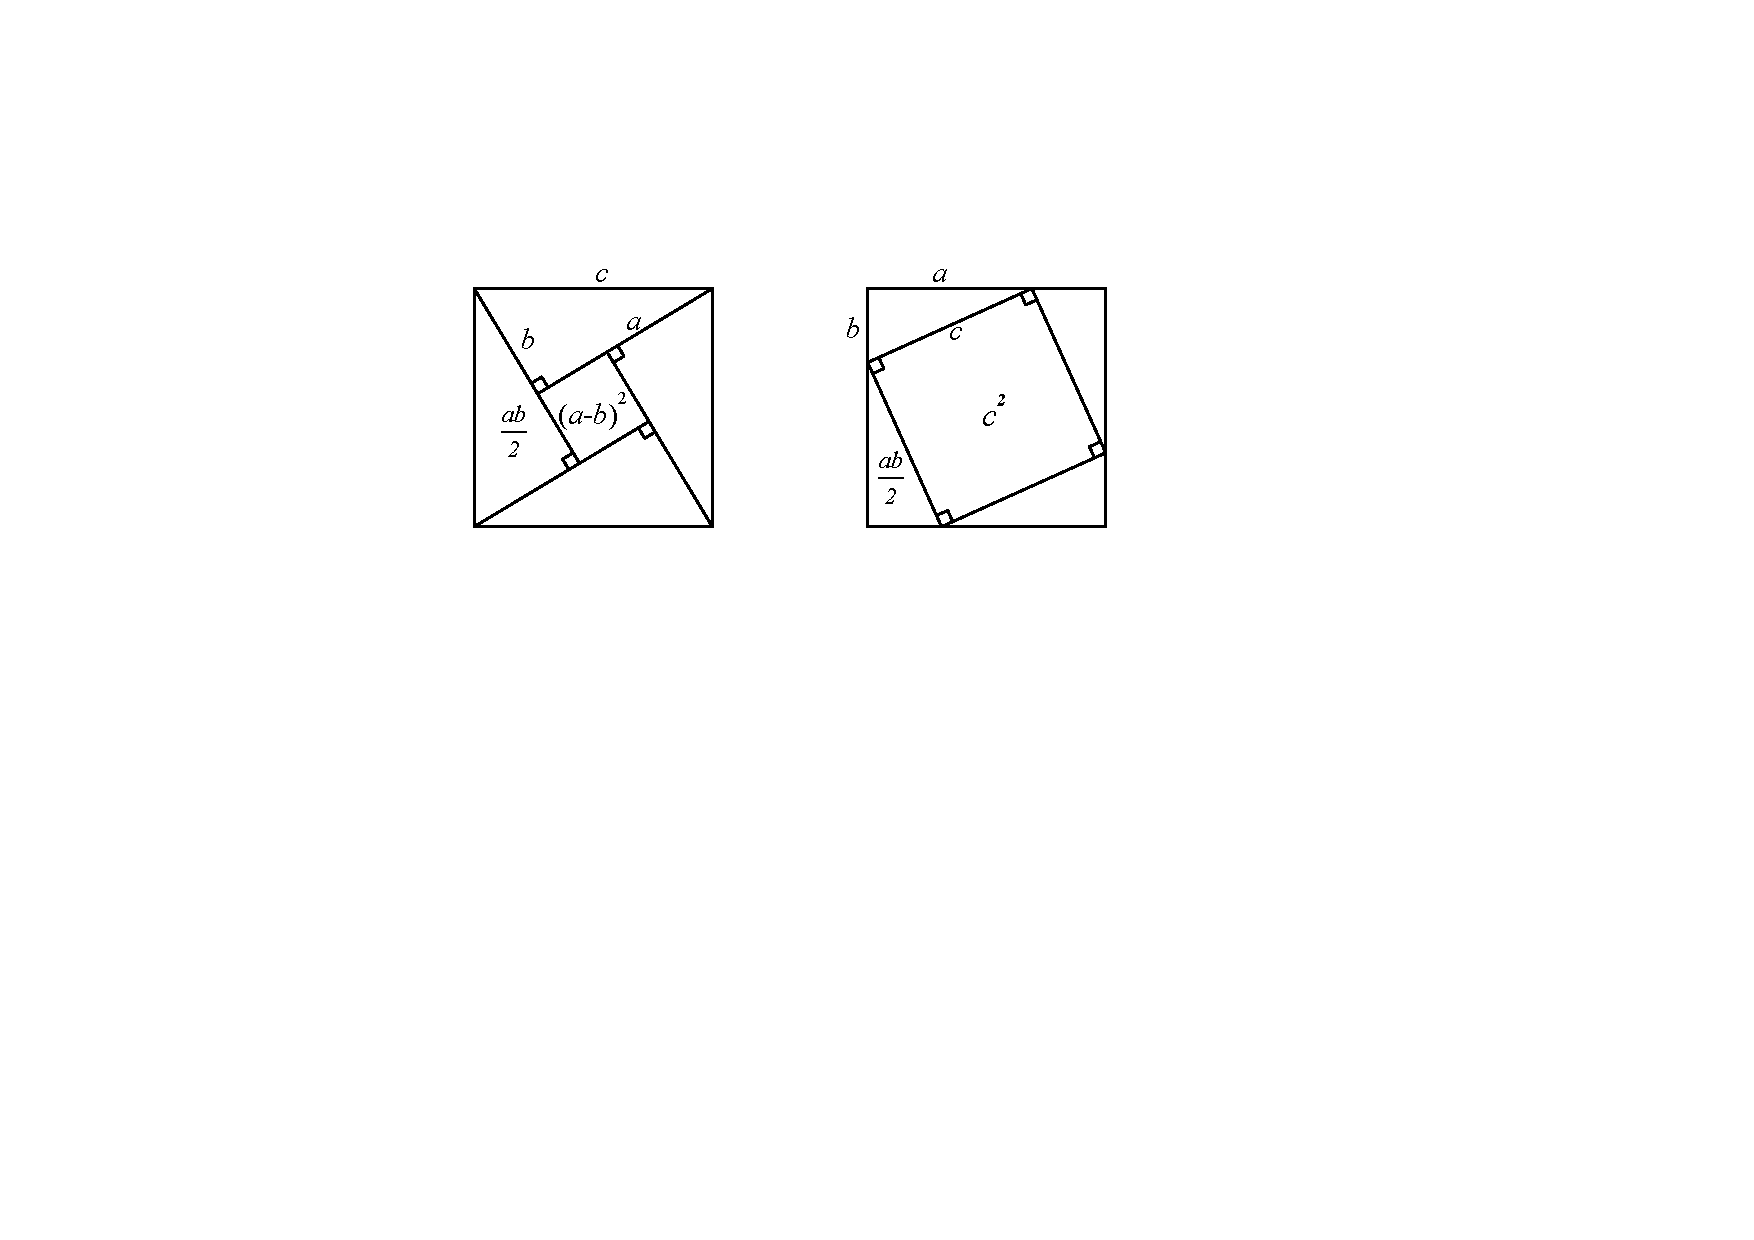
\includegraphics[width=0.7\linewidth]{勾股定理的证明}
\end{figure}  \\
对于左图:$ 4\times \dfrac{1}{2}ab+(a-b)^2=c^2 $. \hspace{2cm} 
对于右图:$ 4\times \dfrac{1}{2}ab+c^2=(a+b)^2 $. 

\item 平方差公式生成各位全是1的整数:
\begin{align*}
    6^2-5^2 &=1\times 11 = 11 \\
    56^2-45^2 &=11\times 101= 1111 \\
    556^2-445^2 &=111\times 1001= 111111 \\
    5556^2-4445^2 &=1111\times 10001=11111111 \\
    55556^2-44445^2 &=11111\times 100001=1111111111 
\end{align*}

\item 一些特殊的平方数:
\begin{align*}
    11^2&=121 \\
    111^2&=12321 \\
    1111^2&=1234321 \\
    11111^2&=123454321 \\
    111111^2&=12345654321 \\
    1111111^2&=1234567654321 \\
    11111111^2&=123456787654321 \\
    111111111^2&=12345678987654321 
\end{align*}
$ 11^2=121,\ 22^2=484 $.\ ($ 11,121,22,484 $
这4个数都是回文数,即从左到右看和从右向左看是一样的。) 
\begin{align*}
    & 12^2=144,\ 21^2=441,\ 13^2=169,\ 31^2=961 \\
    & 112^2=12544,\ 211^2=44521,\ 113^2=12769,\ 311^2=96721 \\
    & 1112^2=1236544,\ 2111^2=4456321,\ 1113^2=1238769,\ 3111^2=9678321 \\
    & 11112^2=123476544,\ 21111^2=445674321,\ 11113^2=123498769,\ 
    31111^2=967894321
\end{align*}
($ n $左右颠倒后,$ n^2 $也左右颠倒。)\\
$ 88^2=7744 $,小学阶段经常喜欢拿这个平方数作为难题。

\item $ \pi\approx 3.141592653 $的分数近似值:$ \dfrac{22}{7} 
\approx 3.142857,\ \dfrac{355}{113}\approx 3.14159292 $. 

\item 三角函数的有界性:$ \theta\in\textbf{R},\ 0\leq |\sin \theta|
\leq 1,\ 0\leq |\cos \theta|\leq 1 $.\\ 比如,$ x\in \textbf{R},\theta 
\in \textbf{R} $,若$ x^2+1=\cos\theta $,则$ x=0,\ \cos\theta=1 $;
若$ x+\dfrac{1}{x}=2\cos\theta $,则$ x=1,\cos\theta=1 $
或$ x=-1,\cos\theta=-1 $. 

\item 设$ \vec{i},\vec{j} $是既不平行又不垂直的
单位向量,有非零向量$ \vec{a}=x_1\vec{i}+y_1\vec{j},
\vec{b}=x_2\vec{i}+y_2\vec{j} $,那么,
$ \vec{a}//\vec{b} $的充要条件仍然是$ x_1y_2-x_2y_1=0 $. 
先不考虑分母为零的情形,这个式子可以变形为$ \dfrac{x_1}{x_2}=\dfrac{y_1}{y_2} $,
说明系数成比例,从相似三角形的角度容易理解向量共线。由于两者都是非零向量,$ x_1=0 $
意味着$ y_1\neq 0,\ x_2=0 $,此时$ \vec{a}//\vec{b}//
\vec{j} $. 当$ x_2=0 $时有类似结论。而$ x_1x_2+y_1y_2=0 $是
$ \vec{a}\perp\vec{b} $
既不充分又不必要条件。因为
\begin{gather*}
    \vec{a}\cdot\vec{b}=(x_1\vec{i}+
    y_1\vec{j})\cdot(x_2\vec{i}+y_2\vec{j})
    =x_1x_2+y_1y_2+(x_1y_2+x_2y_1)\vec{i}\cdot \vec{j}
\end{gather*}

\item 科克雪花曲线(koch snowflake),$ n=1 $时,只有一个边长为1的正三角形,第$ n $次生成后,边数$ N_n=3 \cdot 4^{n-1} $,
每条边的长度 $ T_n=\left(\dfrac{1}{3} \right)^{n-1}  $,
周长$ L_n=N_n \cdot T_n=3\cdot \left( \dfrac{4}{3}\right)^{n-1}  $,可以发散到无穷大,
面积$ A_n =A_1(1+N_1 T_2^2+N_2T_3^2+\cdots +N_{n-1}T_n^2)
=\dfrac{2}{5}\sqrt{3}-\dfrac{3\sqrt{3}}{20}\left(\dfrac{4}{9} \right)^{n-1}  $,是有限的。

\item 秦九韶算法可以大大减少多项式求值时做乘法的次数,因而能提高计算效率,
\begin{align*}
    p_n(x) =&\ a_nx^n+a_{n-1}x^{n-1}+\cdots + a_1x+a_0 \\
    =&\ (\cdots (((a_nx+a_{n-1})x+a_{n-2})x+a_{n-3})x\cdots +a_1)x+a_0
\end{align*}	
由内向外逐层计算。假如需要对不同的多项式求值,那么秦九韶算法是首选。但如果是一个确定的多项式对不同的自变量多次求值,还可以考虑另外一种方法,那就是事先求出这个多项式的全部根,然后将其写成实数范围内的因式分解形式$ a(x-x_1)(x-x_2)\cdots (x-x_r)(x^2+p_1x+q_1)\cdots(x^2+p_sx+q_s) $. 这种方法编程非常简单,而且是可并行的(同时进行多个加、减法运算),而秦九韶算法只能串行。此法的弊端是:如果多项式的系数和自变量都是整数,那么秦九韶算法可以使用计算芯片中的整数运算单元,而因式分解后可能必须使用浮点计算单元。浮点计算的速度比整数慢,而且会存在误差,此时就应该选择秦九韶算法。

\item 交流电的有效值:
\begin{gather*}
I^2=\int_{0}^{T}\left( I_m\sin \omega t\right)^2 \d t
=\dfrac{1}{2}I_m^2 \int_{0}^{T}\left( 1-\cos 2\omega t\right) \d t
=\dfrac{1}{2}I_m^2
\end{gather*}
其中,$ T=\dfrac{2\pi}{\omega} $,所以,有效值是峰值的
$ \dfrac{\sqrt{2}}{2} $倍。即在一个周期内,大小为$ \dfrac{\sqrt{2}}{2}I_m $
的直流电与峰值为$ I_m $交流电,在导体上产生同样的热量。

\item 单摆在小角度摆动时可视为简谐振动,下面用量纲分析法研究单摆的运动周期。
假设单摆的运动周期$ T $与末端质点质量$ m $、摆长$ l $和重力加速度$ g $有关,
且可以写成乘积形式,即$ T=Am^{\alpha}l^{\beta}g^{\gamma} $,
其中$ A $是没有单位的常数,$ T $的单位为秒(s),$ m $的单位为千克(kg),
$ l $的单位为米(m),$ g $的单位为米/秒$ ^2 $(m/s$ ^2 $),等式两端的
单位应该相同,即s=(kg)$ ^\alpha $m$ ^\beta $(m/s$ ^2 $)$ ^\gamma $,于是
$ \begin{cases}
    \alpha=0 \\
    \beta+\gamma =0 \\
    -2\gamma =1
\end{cases} $. 解得
$ \begin{cases}
    \alpha=&\ 0 \\
    \beta=&\ \dfrac{1}{2} \\
    \gamma =&\ -\dfrac{1}{2}
\end{cases} $,所以$ T=A\sqrt{\dfrac{l}{g}} $. 事实上,通过其它研究手段,
可得到$ T=2\pi \sqrt{\dfrac{l}{g}} $. 量纲分析法原理十分简单,但在物理学研究中具有
相当重要的作用。谁在这方面进行深入的思考,谁就能做出很多聪明的研究工作来。

\item 弹簧振子简谐振动$ x=A\sin\left( \sqrt{\dfrac{k}{m}}t\right) $,有阻尼振动
$ x=Ae^{-\xi t}\sin\left( \sqrt{\dfrac{k}{m}}t\right) $. 
请读者分析$ \sqrt{\dfrac{k}{m}} $的单位。

\item 电容充电时,电压随时间的变化:$ U=E\left(1-\e^{-\frac{t}{RC}} \right) $. 
电容放电时,电压随时间的变化:$ U=U_0\e^{-\frac{t}{RC}}$.
$ R $为与电容串联的电阻阻值,$ C $为电容的大小,$ E $为电源的电压,
$ U_0 $为电容放电前的电压。请分析$ \dfrac{t}{RC} $的单位.

\item $ y=A\sin x $可由$ y=\sin x $进行$ y $方向的缩放而来,若$ A\neq 1 $,则无论进行怎样的平移,两者的图像都不可能重合。$ y=Ax^2\ (A\neq 1) $与$ y=x^2 $,靠平移也不可能使两者重合。但对于指数函数$ y=Aa^x=a^{x+\log_a A}\ (a>0,a\neq 1,A>0) $,却能通过平移与$ y=a^x $重合,即$ y $方向的缩放并未改变指数函数图像的形状。同理,因为$ y=\log_a(\omega x)=\log_a \omega+\log_a x \ (\omega>0) $,所以$ x $方向的缩放不改变对数函数图像的形状。

\item 辗转相除法求最大公约数:不断进行带余除法,直到余数为0. \\
求1961和15133的最大公约数。
\begin{align*}
    15133\div \underline{1961} =&\ 7\cdots\cdots \underline{1406} \\
    1961\div \underline{1406} =&\ 1\cdots\cdots \underline{555} \\
    1406\div \underline{555} =&\ 2\cdots\cdots \underline{296} \\
    555\div \underline{296} =&\ 1\cdots\cdots \underline{259} \\
    296\div \underline{259} =&\ 1\cdots\cdots \underline{37} \\
    259\div 37 =&\ 7\cdots\cdots 0
\end{align*}
于是,$ 1961=37\times 53 $和$ 15133=37\times409 $的最大公约数是37.\\
\textbf{注}\ 贝祖(Bezout)等式:设$ a,b $是非零整数,$ d=\gcd(a,b) $,代表$ a,b $
的最大公约数,那么存在整数$ x,y $,满足$ ax+by=d $. 比如,$ a=697,\ b=391,\ d=\gcd(697,391)=17,\ 9\times 697+(-16)\times 391=17 $. 对于上面的1961和15133,有
$ 7\times 15133+(-54)\times 1961=37 $. 

\item 原命题:若$ p $,则$ q $;
逆命题:若$ q $,则$ p $;\\
否命题:若$ \neg p $,则$ \neg q $;
逆否命题:若$ \neg q $,则$ \neg p $. 

\item 集合的3个特征:确定性、互异性、无序性。

\item $ A \subseteq B $:集合$ A $为集合$ B $的子集(可能有$ A=B $)。\\
$ \ \ A \subsetneqq B $:集合$ A $为集合$ B $的真子集(不能有$ A=B $)。\\
空集($ \varnothing $)是任何集合的子集。\\
只含有限个元素的集合$ A $叫有限集,用$ \mathrm{card}(A) $表示有限集合$ A $
中的元素个数,那么
\begin{gather*}
    \mathrm{card}(A\cup B)=\mathrm{card}(A)+\mathrm{card}(B)-
    \mathrm{card}(A\cap B)
\end{gather*}

\item “$ (x-2)^2+(y-3)^2>1 $”是“$ |x-2|+|y-3|>1 $”的“充分非必要”条件。\\
\textbf{解}\ 前者可看成点$ (x,y) $到点$ (2,3) $的距离大于1,相当于直角三角形的斜边大于1,
而后者则意味着两条直角边之和大于1,所以前者一定是充分的。取$ |x-2|=|y-3|=0.6 $,
可以说明前者不是必要的。\\
\textbf{注}\ 本题有向量范数的背景,
设$ n $维向量$ \vec{v}=(v_1,v_2,\cdots,v_n) $,那么向量的$ p $-范数
($ p > 0 $)定义为:$ ||\vec{v}||_p
=\left(\sum\limits_{i=1}^n |v_i|^p\right)^{\frac{1}{p}} $. 
范数也有三角不等式,若$ p>1 $,则
\begin{align*}
    ||\vec{x}+\vec{y}||_p\leq
    ||\vec{x}||_p+||\vec{y}||_p
\end{align*}
其实就是闵可夫斯基(Minkowski)不等式。

\item $ \sqrt{2} $是无理数。\\
\textbf{证}\ 假设$ \sqrt{2} $是有理数,那么它可以表示成两个互质整数的商,即$ \sqrt{2}=
\dfrac{a}{b} $,平方后可得$ 2b^2=a^2 $. 如果$ a $是奇数,那么$ a^2 $也是奇数,就不可能等于$ 2b^2 $
这个偶数,所以$ a $必然是偶数。假设$ a=2k $,那么$ 2b^2=(2k)^2=4k^2,b^2=2k^2, $同理可得$ b $
也是偶数,于是$ a,b $同为偶数,这与两者互质的条件矛盾,所以$ \sqrt{2} $不能表示成两个互质整数的商。同样的方法可证明$ \sqrt[n]{2} $不是有理数。\\
\textbf{推广}:$ k\in \textbf{N}^+ $,如果$ \sqrt{k} $不是整数,
那么$ \sqrt{k} $是无理数。

\item 质数有无限多个。\\
\textbf{证}\ 用反证法:假设质数只有有限个,将它们依次记为$ p_1,p_2,\cdots p_n $,
令$ P=p_1p_2\cdots p_n+1 $. 如果$ P $是质数,那就又创造了一个新的、更大的质数,
与“质数有限”的假设矛盾。如果$ P $不是质数(比如$ P = 2\times 3\times 5\times 7\times 11\times 13+1=30031 $),那它一定可以分解成若干个质因子的乘积($ 30031=59\times 509 $),
而$ P $除以$ p_1,p_2,\cdots p_n $中的任意一个数的余数都是1,
说明$ p_1,p_2,\cdots p_n $都不是$ P $的质因子,所以$ P $的质因子(59和509)都是新的质数,
同样与“质数有限”的假设矛盾。综上所述,质数有无限多个。\\
\textbf{注1}:对于任意大于1的整数$ n $,存在正整数$ x_1,x_2,\cdots,
x_n $,满足
\begin{align*}
    \dfrac{1}{x_1}+\dfrac{1}{x_2}+\cdots+\dfrac{1}{x_n}+
    \dfrac{1}{x_1x_2\cdots x_n}=1
\end{align*}
容易算出$ x_1=2,\ x_2=3,\ x_3=7,\cdots $,有趣的是,$ x_n=
x_1x_2\cdots x_{n-1}+1 $,与上面的$ P $的构造方式可谓完全一致,
请读者用归纳法证明$ x_n $的递推表达式。很容易产生进一步地思考:
$ x_n $会不会全都是质数?编程验证一下就知道答案是否定的,
$ x_5=1807=13\times 139 $不是质数。那么我们可以再做另一个相反的猜想,是否从$ x_7 $开始,全都是合数?不过$ x_n $的增长速度太快,$ x_{11}\approx 2.74\times 10^{208} $,
$ x_{12} $就超过了双精度浮点数所能表示的最大值(约
$ 1.797\times 10^{308} $,想研究前述猜想,就需要
一些特殊的编程技巧来处理这些巨大的整数。)\\
\textbf{注2}:如下的连续$ n-1 $个正整数全都是合数,
\begin{align*}
    n!+2,\ n!+3,\ n!+4,\cdots,n!+n
\end{align*}
因为它们依次能被$ 2,3,4,\cdots,n $整除。同时也说明,
相邻两个质数之间的间隔可以任意大。 \\
\textbf{注3}:威尔逊定理:当且仅当$ n $是质数时,$ n $能整除$ (n-1)!+1 $. (该定理可由费马小定理证明。) 

\item $ ^* $ 求证:当$ n>2 $时,$ n $和$ n! $之间至少存在一个质数。\\
\textbf{证}\ 首先,相邻的两个自然数是互质的,那么$ n!-1 $与$ n! $是互质的。
$ 2,3,\cdots,n $这连续$ n-1 $个正整数都是$ n! $的因子,同时,都不是$ n!-1 $的因子,
否则$ n!-1 $与$ n! $就有大于1的公因子,与两者互质矛盾。设$ n!-1 $的一个质因子为
$ p\ (p\leq n!-1) $,那么$ n<p\leq n!-1<n! $,所以,
$ n $和$ n! $之间至少存在一个质数。

事实上有更强的Bertrand-Chebyshev(伯特兰-车比雪夫)定理:$ \forall n\in \textbf{N}^+,n\geq 2 $,区间$ (n,2n) $内至少存在一个质数。

\item 已知$ a,b,c $都在区间$ (0,1) $内,求证:$ (1-a)b,(1-b)c,(1-c)a $
不能同时大于$ \dfrac{1}{4} $.  \\
\textbf{证}\ 用反证法:假设$ (1-a)b,(1-b)c,(1-c)a $同时大于$ \dfrac{1}{4} $,则
\begin{align*}
    \dfrac{1-a+b}{2} \geq &\ \sqrt{(1-a)b}>\dfrac{1}{2} \\
    \dfrac{1-b+c}{2} \geq &\ \sqrt{(1-b)c}>\dfrac{1}{2} \\
    \dfrac{1-c+a}{2} \geq &\ \sqrt{(1-c)a}>\dfrac{1}{2}      
\end{align*}
以上三式相加可得:$ 0>0 $,产生矛盾。 

\item  一个笑话,同时也是一个知识点:如果一个pizza的半径是z,高度是a,
则它的体积为pizza. (注:pi就是指$ \pi $.)

\item $ ^* $ 无穷正项数列$ \{a_n\} $满足$ (a_{n+1}+n)a_n=1,n\in 
\textbf{N}^+ $,求证:$ \{a_n\} $所有项均为无理数。

\end{itemize}

\section{丑陋的题}
\begin{enumerate}[label={【\textbf{例\thechapter.\arabic*}】},
 leftmargin=\inteval{\myenumleftmargin}pt,
 itemsep=\inteval{\myenumitempsep}pt,
 itemindent=\inteval{\myenumitemindent}pt]
\item (2016,上海春季高考)
对于数列$ \{a_n\} $与$ \{b_n\} $,若对数列$ \{c_n\} $的每一项$ c_k $,均有
$ c_k=a_k $或$ c_k=b_k $,则称数列$ \{c_n\} $是$ \{a_n\} $与$ \{b_n\} $
的一个“并数列”。\\
(1)数列$ \{a_n\} $与$ \{b_n\} $的前三项分别为$ a_1=1,a_2=3,a_3=5,b_1=1,b_2=2,
b_3=3 $,若数列$ \{c_n\} $是$ \{a_n\} $与$ \{b_n\} $的一个“并数列”,
求所有可能的有序数组$ (c_1,c_2,c_3) $. \\
(2)已知数列$ \{a_n\} $、$ \{c_n\} $均为等差数列,$ \{a_n\} $的公差为1,
首项为正整数$ t $ ,$ \{c_n\} $的前10项和为$ -30 $,前20项和为$ -260 $,
若存在唯一的数列$ \{b_n\} $,使得$ \{c_n\} $是$ \{a_n\} $与$ \{b_n\} $
的一个“并数列”,求$ t $的值所构成的集合。\\
\textbf{解}\ (1)\ $ (1,3,5),(1,2,3),(1,2,5),(1,3,3) $. \\
(2)$ a_n=n-1+t $,是单调递增数列,$ c_n=-2n+8 $是单调递减数列,
若$ a_n=c_n $,则$ n-1+t=-2n+8,\ t=9-3n\geq 1,\ n=1,2 $,当$ n=1 $时,$ t=6 $;
当$ n=2 $时,$ t=3 $. 所以,从某3项开始,$ a_n=c_n $永远不会成立,
只能是$ b_n=c_n $. 如果$ a_1=t=6=c_1 $,那么$ b_1 $便能随意取值;
如果$ a_2=t+1=4=c_2 $,那么$ b_2 $便能随意取值,这两种情况都会让$ \{b_n\} $不唯一,
所以,正整数$ t $的取值集合为$ \{t\in \textbf{N}^+|t\neq 3,t\neq 6\} $. \\
\textbf{点评}:此题第(2)问比较费解,考察的也不是高中数学的主要知识点,
像是在考阅读理解。\\
\\
凡是考察函数的题目,一旦出现绝对值、分段、$ \max $ 、$ \min $、取整,
就很容易成为繁琐的、丑陋的题目。

\item 已知实数$ a,b $满足$ a=10^{7-a},\ \lg b=10^{4-\lg b}-3 $,求$ ab $的值。\\
\textbf{解}\ 
\begin{align*}
    a=10^{7-a} \Rightarrow \lg a=7-a \Rightarrow &\  a+\lg a=7 \\
    \lg b=10^{4-\lg b}-3 \Rightarrow 10^{4-\lg b}+(4-\lg b)=7 \Rightarrow & \ 
    10^{4-\lg b}+\lg (10^{4-\lg b})=7 
\end{align*}
因为$ x+\lg x $是$ (0,+\infty) $上的增函数,所以$ a=10^{4-\lg b},\ \lg a=4-\lg b,\ 
\lg a+\lg b=4,\ ab=10^4 $. \\
\textbf{点评}:此题矫揉造作,毫无意义。

\item 定义函数$ f(x)=-x\ln x+x^2-2ax+k \ (k>0) $,当$ x>0 $时,$ f(x) $的最小值为0,
求$ k-4a $的最小值。\\
\textbf{解}\ $ f'(x)=-\ln x-1+2x-2a,\ f''(x)=-\dfrac{1}{x}+2 $,所以,$ f'(x) $
在$ (0,\dfrac{1}{2}) $单调递减,在$ (\dfrac{1}{2},+\infty) $上单调递增,$ f'(x) $
在$ \dfrac{1}{2} $处取得极小值。\\
I.若$ f'(\dfrac{1}{2})=\ln2-2a\geq 0 $,那么$ f(x) $在$ (0,+\infty) $上单调递增,
$ f(x)_{\min}=\lim\limits_{x\to 0}f(x)=k=0 $,与题目中的$ k>0 $矛盾。\\
II.若$ \ln2-2a < 0 $,于是存在$ 0<x_1<\dfrac{1}{2}<x_2 $,满足$ f'(x_1)=f'(x_2)=0 $,
显然,$ x_1 $是$ f(x) $的极大值点,$ x_2 $是$ f(x) $的极小值点,同时有$ f(x_2)=0 $,
\begin{align*}
    \begin{cases}
        & f'(x_2)=-\ln x_2-1+2x_2-2a=0  \quad\mycircled{1} \\
        & f(x_2)=-x_2\ln x_2+x_2^2-2ax_2+k=0 \quad\mycircled{2}
    \end{cases}
\end{align*}
由\mycircled{1}得:$ 2a=-\ln x_2-1+2x_2 $,代入\mycircled{2}可得:
$ k=x_2^2-x_2 $,所以$ k-4a=x_2^2-5x_2+2\ln x_2+2 $,容易算出$ g(x)=x^2-5x+
2\ln x+2 $在$ \Big(\dfrac{1}{2},+\infty\Big) $上的最小值是
$ g(2)=2\ln 2-4 $. \\
\textbf{点评}:绕的弯子实在太多,需要多次求导,还需要用到
$ \lim\limits_{x\to 0} x\ln x=0 $这个对高中生而言不太熟悉的极限。\\

\end{enumerate}
\cleardoublepage
%
%\chapter{自我检测}
%~\newpage

%\ChuBanbookfalse
%\ChuBanbooktrue
%\ifChuBanbook 
